\chapter{Alignment}
% Fonte: Xiao e Zhu, Foundations of Large Language Models,
% Capitolo 4, pp. 155--186.
%
% Dipendenze da inserire nel preambolo del documento principale:
% \usepackage{amsmath,amssymb,graphicx}
%
% Le equazioni conservano la numerazione del libro.
% Le spiegazioni aggiuntive sono contrassegnate come chiarimenti
% o esempi pratici.
%
% Le figure compilano anche in assenza dei file immagine:
% in questo caso viene visualizzato un riquadro segnaposto.



\section{Alignment}

\subsection*{Introduzione e motivazioni}

Nel Natural Language Processing (NLP), il termine
\emph{Alignment} ha assunto significati differenti a seconda
dell'ambito e del periodo storico. Nel NLP tradizionale indicava
principalmente l'individuazione di corrispondenze fra elementi di
due insiemi: per esempio, l'associazione fra le parole di una frase
in cinese e quelle della corrispondente frase in inglese.

Nel contesto dei Large Language Models (LLM), il termine viene
utilizzato in un senso più ampio.

\begin{definition}{Alignment di un LLM}
L'Alignment è il processo attraverso il quale si cerca di rendere
gli output di un modello coerenti con le aspettative umane,
comprendendo le istruzioni, gli obiettivi, le intenzioni,
i valori e le preferenze degli utenti.
\end{definition}

Il problema nasce dal fatto che un modello può generare risposte
che non corrispondono agli obiettivi o al contesto desiderati
dall'utente. In particolare:

\begin{itemize}
    \item un modello sottoposto soltanto a Pre-training può non
    saper seguire le istruzioni, perché non è stato addestrato
    esplicitamente a farlo;

    \item un modello può produrre contenuti dannosi oppure
    riprodurre i bias presenti nei dati di addestramento;

    \item una risposta può risultare linguisticamente plausibile,
    ma non essere appropriata rispetto alle aspettative,
    ai valori o alle norme sociali rilevanti.
\end{itemize}

L'obiettivo generale è quindi ottenere modelli i cui output siano
\textbf{accurati, pertinenti, sicuri e non discriminatori}.

\paragraph{Perché il solo Pre-training non è sufficiente.}
In linea teorica, un insieme di dati sufficientemente ampio,
rappresentativo di tutti i task e coerente con le preferenze umane
potrebbe consentire di ottenere un modello già adeguatamente
allineato mediante il solo Pre-training.

Nella pratica, tuttavia, è quasi impossibile raccogliere dati
che coprano tutti i task e rappresentino adeguatamente la
complessità delle preferenze umane (cioè gli obiettivi, le intenzioni ecc... di tutti gli umani). 
Per questa ragione,
l'Alignment costituisce una fase necessaria nello sviluppo
degli LLM descritti nel capitolo.

Si distinguono \textbf{due grandi obiettivi dell'Alignment}:

\begin{itemize}
    \item \textbf{Instruction Alignment}: orientare il modello
    a generare output conformi alle istruzioni dell'utente,
    principalmente mediante Supervised Fine-Tuning;

    \item \textbf{Human Preference Alignment}: ha l'obiettivo di allineare il comportamento del modello alle preferenze umane.
    Principalmente mediante Reinforcement Learning basate sul feedback umano.
\end{itemize}

I due approcci rispondono a obiettivi diversi, ma vengono
comunemente utilizzati insieme.



\newpage
\subsection{Panoramica dell'Alignment degli LLM}

Come anticipato, l’Alignment persegue due obiettivi principali: consentire al modello di seguire le istruzioni dell’utente e renderne il comportamento coerente con le preferenze umane. Per raggiungerli, si possono utilizzare i tre approcci che descriveremo di seguito
\subsubsection*{Fine-tuning con dati annotati}

Il primo approccio consiste nel proseguire l'addestramento di un
modello pre-addestrato utilizzando dati annotati, così da adattarlo
a task specifici.

Nel \textbf{Supervised Fine-Tuning (SFT)}, il dataset contiene
istruzioni associate agli output attesi. Rispetto al dataset
di Pre-training, quello di SFT è generalmente molto più piccolo,
ma anche più specializzato.

Per esempio, un modello sottoposto a Fine-tuning su coppie
domanda--risposta può imparare a rispondere anche a domande
non presenti esplicitamente nel dataset di SFT.

Questo approccio è particolarmente adatto quando:

\begin{itemize}
    \item la relazione fra input e output è relativamente facile
    da descrivere;

    \item è possibile annotare gli esempi in modo sufficientemente
    chiaro e affidabile.
\end{itemize}

\subsubsection*{Fine-tuning mediante un Reward Model}

Il secondo approccio utilizza un \textbf{Reward Model}.

Valori e aspettative umane sono difficili da formalizzare:
anche una persona può avere difficoltà a spiegare precisamente
che cosa renda una risposta eticamente corretta o culturalmente
appropriata. Di conseguenza, non sempre è semplice costruire
esempi supervisionati che descrivano completamente il
comportamento desiderato.

In questi casi, il problema non consiste soltanto nell'adattare
il modello a un insieme limitato di esempi. Occorre anche
fornirgli un criterio per distinguere gli output maggiormente
coerenti con le preferenze umane.

\begin{definition}{Reward Model}
Un Reward Model è un modello che assegna un punteggio agli output
di un LLM, con l'obiettivo di valutarne la corrispondenza ai
comportamenti e alle preferenze desiderati.
\end{definition}

Il Reward Model può essere addestrato a partire da dati di
preferenza umana e successivamente impiegato per guidare
l'aggiornamento dell'LLM.

L'analogia proposta dal testo è quella di un insegnante che
fornisce feedback a uno studente: il modello viene incentivato
a produrre risposte che ricevono valutazioni migliori.

Questo conduce al
\textbf{Reinforcement Learning from Human Feedback (RLHF)},
che permette di affrontare aspetti del comportamento umano
e delle norme sociali difficili da esprimere mediante sole
coppie input--output.

Quindi questo Fine-Tuning mediante Reward Model è un tipo di Fine-Tuning che utilizza il Reinforcement Learning from Human Feedback.

\subsubsection*{Alignment durante l'Inference}

Il terzo approccio interviene durante l'\textbf{Inference},
senza richiedere ulteriori aggiornamenti dei parametri.

Un primo esempio è il \textbf{Prompting}: modificando il prompt,
si può orientare dinamicamente il comportamento di un modello
verso task differenti, con un costo contenuto.

Un secondo esempio è il \textbf{rescoring degli output}:
si generano più risposte e si applica un sistema di valutazione
che simula il feedback umano, dando priorità agli output
che ricevono punteggi migliori.

\paragraph{Sequenza tipica di sviluppo.}
I tre approcci vengono frequentemente applicati in successione:
dopo il Pre-training si esegue SFT, poi RLHF e infine si utilizzano
tecniche di Prompting durante l'Inference.

Lo sviluppo viene così suddiviso, a grandi linee, in una fase
di \textbf{Pre-training} e una fase di \textbf{Alignment}.
Nella prospettiva del testo, quest'ultima comprende sia gli
interventi di addestramento sia quelli applicati durante
l'Inference.

\begin{figure}[h]
    \centering
    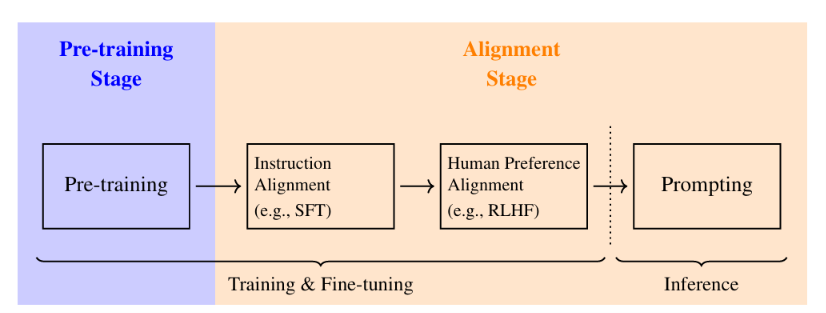
\includegraphics[width=0.8\textwidth]{_files/_images/placeholder_figura_4_1.png}
    \caption{Schema del processo di sviluppo
    pre-train-then-align. Il Pre-training mediante next-token
    prediction è seguito da due tipi di Fine-Tuning (SFT e Reward Model), che consentono l'allineamento.
    SFT e RLHF fanno parte della fase di Post-Training, in generale in Fine-Tuning, fa parte della fase di Post-Training.
    Mentre l'inferenza è la terza grande fase, dopo il Pre-Training e il Fine-Tuning}
    \label{fig:alignment-pipeline}
\end{figure}

\subsection{Instruction Alignment}
Ricordiamo da prima che l'Instruction Alignment ha come obiettivo di:
\begin{center}
    Orientare il modello a generare output conformi alle istruzioni dell'utente
\end{center}


Un prompt è spesso composto da un'\textbf{istruzione} e da un input
fornito dall'utente. Il modello deve comprendere l'istruzione
e applicarla correttamente all'input.

\begin{definition}{Instruction-following ability}
L'Instruction-following ability è la capacità di un LLM
di eseguire un task seguendo le istruzioni contenute
nel prompt dell'utente.
\end{definition}

Si consideri l'esempio del libro, qui espresso in italiano:

\begin{quote}
\textbf{Istruzione:} Riassumi questo testo in tre frasi.

\textbf{Input:} Un articolo sull'ora legale, sulla sua
introduzione in Germania nel 1916 e sullo spostamento
degli orologi durante il periodo estivo.

\textbf{Output atteso:} Un riassunto dell'articolo in tre frasi.
\end{quote}

Tuttavia,gli LLMs sono tipicamente allenati per la next-token prediction rispetto alla generazione dell'output tramite delle istruzioni.
Applicare un LLMs pre-allenato all'esempio sopra, porterebbe probabilmente al modello di continuare l'articolo in input invece di sintetizzare i punti principali.
L'obiettivo dell'instruction alignment è \textbf{di orientare l'LLM a rispondere accuratamente alle istruzioni e intenzioni dell'utente}.


\subsubsection{Supervised Fine-Tuning}

Un approccio diretto per orientare l'LLM a seguire le istruzioni dell'utente è di fare fine-tuning del modello utilizzando coppie annotate di input-output.

Diversamente dal normale addestramento linguistico, l'obiettivo
non è massimizzare la probabilità dell'intera sequenza,
ma la probabilità della parte di risposta, condizionata
al prefisso che contiene la richiesta.

\begin{definition}{Dataset di SFT}
Un dataset di SFT è un insieme di coppie $(x,y)$, nel quale
$x$ contiene l'istruzione ed eventualmente l'input dell'utente,
mentre $y$ rappresenta una risposta corretta a tale richiesta.
\end{definition}

Il testo introduce questa raccolta come $S$ e utilizza poi
$D$ nelle formule dell'obiettivo di addestramento.

Un singolo dataset può contenere esempi relativi a task diversi.
Gli esempi proposti dal libro comprendono:

\begin{itemize}
    \item \textbf{Riassunto}: un'istruzione che richiede di
    riassumere un articolo sulla crescita dell'energia solare,
    associata al relativo riassunto;

    \item \textbf{Estrazione di informazioni}: un'istruzione
    che richiede di estrarre dati finanziari da una relazione,
    associata a un output che riporta ricavi pari a
    $10$ milioni di dollari e un margine di profitto del $15\%$;

    \item \textbf{Classificazione}: un'istruzione che richiede
    di classificare come spam o non spam un'email che annuncia
    la vincita di un buono da $500$ dollari,
    associata all'etichetta \emph{Spam};

    \item \textbf{Assistenza tecnica}: una richiesta di soluzione
    per un computer lento e soggetto a blocchi,
    associata a una procedura di controllo e risoluzione.
\end{itemize}

Questo consente di adattare un unico modello a più task
contemporaneamente.

\paragraph{Notazione e obiettivo.}
Siano
\[
x=x_0\ldots x_m,
\qquad
y=y_1\ldots y_n
\]
la sequenza di input e quella di output.

Qui $x_i$ e $y_i$ indicano token; $x$ contiene, per esempio,
l'istruzione e l'input dell'utente.

Considera un LLM con parametri di pre-training $\hat{\theta}$. L'obiettivo di SFT è massimizzare la probabilità dell'output $y$ dato l'input $x$
\[
\tilde{\theta}
=
\operatorname*{arg\,max}_{\hat{\theta}^{+}}
\sum_{(x,y)\in D}
\log \Pr_{\hat{\theta}^{+}}(y\mid x).
\tag{4.1}
\]

Nella formula:

\begin{itemize}
    \item $D$ è il dataset di Fine-tuning;

    \item $\hat{\theta}^{+}$ indica i parametri ottenuti
    modificando quelli pre-addestrati, si parte quindi da quelli pre-addestrati e si modificano per massimizzare la probabilità;

    \item $\tilde{\theta}$ indica i parametri ottimizzati
    mediante Fine-tuning.
\end{itemize}

\textbf{L'obiettivo quindi è trovare i parametri ottimizzati \(\tilde{\theta}\), partendo dai parametri di pre-training \(\hat{\theta}\), che massimizzano la probabilità di generare l'output desiderato \(y\), dato l'input \(x\).}
Durante l'SFT, vogliamo che il modello impari ad assegnare un'alta probabilità alla risposta corretta, quando riceve la domanda corrispondente.

Per alleggerire la notazione, il testo utilizza successivamente
$\theta$ al posto di $\hat{\theta}^{+}$. Resta essenziale che
\textbf{il Fine-tuning inizi dai parametri pre-addestrati},
anziché da un'inizializzazione casuale.


\paragraph{Fattorizzazione autoregressiva.}

La log-probabilità della risposta si scompone nella somma
delle log-probabilità dei suoi token. Vediamo nel dettaglio
come si ottiene questa espressione.

Consideriamo una risposta $y$ composta da $n$ token:
\[
y = (y_1, y_2, \ldots, y_n).
\]

Vogliamo calcolare la probabilità che il modello generi
l'intera risposta $y$, dato l'input $x$:
\[
\Pr_{\theta}(y \mid x)
=
\Pr_{\theta}(y_1, y_2, \ldots, y_n \mid x).
\]

\textbf{Passaggio 1: regola della catena delle probabilità.}

Applicando la regola della catena delle probabilità,
possiamo esprimere la probabilità dell'intera sequenza
come prodotto di probabilità condizionate:

\[
\begin{aligned}
\Pr_{\theta}(y \mid x)
={}& \Pr_{\theta}(y_1 \mid x)\\
&\cdot \Pr_{\theta}(y_2 \mid x,y_1)\\
&\cdot \Pr_{\theta}(y_3 \mid x,y_1,y_2)\\
&\cdots\\
&\cdot \Pr_{\theta}(y_n \mid x,y_1,\ldots,y_{n-1}).
\end{aligned}
\]

Questo è coerente con il funzionamento autoregressivo
del modello: la probabilità di ciascun token dipende
dall'input completo $x$ e dai token precedenti
della risposta.

Introducendo la notazione
\[
y_{<i} = (y_1,\ldots,y_{i-1}),
\]
che indica i token della risposta precedenti
alla posizione $i$, possiamo scrivere:

\[
\boxed{
\Pr_{\theta}(y \mid x)
=
\prod_{i=1}^{n}
\Pr_{\theta}(y_i \mid x,y_{<i})
}
\]

\textbf{Passaggio 2: applicazione del logaritmo.}

Applichiamo il logaritmo a entrambi i membri:

\[
\log \Pr_{\theta}(y \mid x)
=
\log \left(
\prod_{i=1}^{n}
\Pr_{\theta}(y_i \mid x,y_{<i})
\right).
\]

Ricordiamo la proprietà dei logaritmi:
\[
\log(a \cdot b) = \log a + \log b.
\]

Il logaritmo di un prodotto diventa quindi
una somma di logaritmi. Otteniamo:

\[
\boxed{
\log \Pr_{\theta}(y\mid x)
=
\sum_{i=1}^{n}
\log \Pr_{\theta}(y_i\mid x,y_{<i})
}
\tag{4.2}
\]

Quindi, \textbf{la probabilità della risposta completa
è il prodotto delle probabilità condizionate dei token,
mentre la log-probabilità della risposta completa
è la somma delle loro log-probabilità}.

\medskip




\paragraph{Chiarimento sul segno dell'obiettivo.}
In un passaggio discorsivo il libro parla di
``minimizzare la log-probabilità condizionata''.
Le equazioni e l'obiettivo descritto richiedono invece di
\textbf{massimizzare la log-probabilità}, oppure,
equivalentemente, di minimizzarne l'opposto:
\[
\mathcal{L}_{\mathrm{SFT}}(\theta)
=
-\sum_{(x,y)\in D}
\sum_{i=1}^{n}
\log \Pr_{\theta}(y_i\mid x,y_{<i}).
\]
Quest'ultima espressione esplicita il collegamento con la loss.
\[
\boxed{\tilde{\theta}=\arg\min_\theta\mathcal{L_{SFT}}(\theta)}
\]
\begin{observation}{Teacher Forcing}
Durante il Supervised Fine-Tuning si utilizza la tecnica del
\textbf{Teacher Forcing}: per predire il token $y_i$, il modello
riceve come contesto l'input $x$ e i \textbf{token corretti
precedenti} $y_{<i}$, presi direttamente dal dataset.

Anche se il modello assegnasse una probabilità maggiore a un
token errato, per la predizione successiva verrebbero comunque
utilizzati i token corretti della risposta.

Questo è possibile perché, durante il training, la risposta
corretta $y$ è nota. Durante l'\textbf{inferenza}, invece,
il modello non conosce $y$ e deve utilizzare come contesto
i token che ha effettivamente generato.

\end{observation}


\paragraph{Concatenazione di input e output.}

Il problema appena introdotto non coincide con il problema standard di
\textit{Language Model Training}, poiché l'obiettivo non è massimizzare
la probabilità di tutti i token di una sequenza, bensì
\textbf{massimizzare la probabilità della risposta $y$, condizionatamente
all'input $x$}.

Nel problema standard di \textit{Language Model Training}, già
affrontato durante lo studio del Pre-Training, l'obiettivo è infatti
massimizzare la log-likelihood delle intere sequenze presenti
nel dataset di addestramento:

\begin{equation*}
    \hat{\theta}
    =
    \arg\max_{\theta}
    \sum_{x \in \mathcal{D}}
    \mathcal{J}_{\theta}(x)
\end{equation*}

Nel Supervised Fine-Tuning (SFT), invece, non siamo interessati
a massimizzare la probabilità dell'intera sequenza composta
dall'input e dalla risposta, ma soltanto quella della risposta
corretta, dato l'input.

Per poter \textbf{ricondurre il problema di SFT alla formulazione
standard del Language Model Training}, possiamo sfruttare la
fattorizzazione della probabilità congiunta e applicare un
opportuno mascheramento della loss.

Vediamo quindi i passaggi necessari.

Si concatenano le due sequenze:
\[
\mathrm{seq}_{x,y}=[x,y].
\]

La chain rule fornisce
\[
\begin{aligned}
\log \Pr_{\theta}(\mathrm{seq}_{x,y})
&=
\log \Pr_{\theta}(x,y)\\
&=
\underbrace{\log \Pr_{\theta}(x)}_{
    \text{contributo escluso dalla loss}}
+
\underbrace{\log \Pr_{\theta}(y\mid x)}_{
    \text{contributo utilizzato nella loss}}.
\end{aligned}
\tag{4.3}
\]

Il primo termine riguarda la generazione dell'input;
il secondo riguarda la generazione della risposta
condizionata all'input.

L'implementazione descritta dal libro procede così:

\begin{enumerate}
    \item si esegue il \textbf{forward pass} sulla sequenza
    concatenata, come in un normale modello autoregressivo;

    \item nel calcolo della loss si annullano i contributi
    associati alla predizione dei token di $x$;

    \item il \textbf{backward pass} utilizza quindi soltanto
    la loss relativa alla parte di output.
\end{enumerate}

Questa operazione viene comunemente descritta come
\textbf{masking della loss}.

Il testo riscrive pertanto l'obiettivo nella forma
\[
\tilde{\theta}
=
\operatorname*{arg\,max}_{\theta}
\sum_{(x,y)\in D}
\log \Pr_{\theta}(\mathrm{seq}_{x,y}).
\tag{4.4}
\]

\paragraph{Chiarimento sulla notazione della formula (4.4).}
La formula va interpretata con il masking appena descritto.
La log-probabilità congiunta ordinaria contiene anche
$\log \Pr_{\theta}(x)$; l'obiettivo effettivamente utilizzato
in SFT ne esclude il contributo.

Non si impone matematicamente che
$\log \Pr_{\theta}(x)=0$: si impone che il suo contributo
alla funzione di addestramento sia nullo.

Inoltre, i token dell'input restano disponibili come contesto
per predire la risposta. Escludere la loss sull'input
non significa rimuovere l'input dall'elaborazione.

\paragraph{Dal single-round al multi-round.}
La formulazione precedente descrive un problema
\textbf{single-round}: a una richiesta segue una risposta,
senza ulteriori interazioni.

Viene detta single-round, perchè il dataset di fine-tuning è definito come:
\[
D=\{(x_1,y_1),(x_2,y_2),\ldots,(x_N,y_N)\}
\]
Quindi il modello viene addestrato a massimizzare:
\[
\tilde{\theta}=\arg\max_\theta
\sum_{(x,y)\in D}\log P_\theta(y\mid x)
\]

Il punto è che ogni risposta viene appresa in funzione della singola richiesta, senza considerare esplicitamente i turni precedenti di una conversazione.


In una conversazione \textbf{multi-round}, invece,
ogni risposta dipende sia dalla richiesta corrente
sia dalla storia precedente.
E quindi gli esempi che contiene il dataset multi-round \textbf{contengono intere osservazioni}

\begin{figure}[h]
    \centering
    
\includegraphics[width=0.8\textwidth]{_files/_images/conversation.png}
    \caption{SFT di un modello conversazionale.
    La sequenza alterna interventi dell'utente e risposte
    del chatbot..}
    \label{fig:sft-conversazionale}
\end{figure}

Il punto rilevante è che ogni risposta richiede di tenere conto
delle informazioni accumulate nei turni precedenti.

Considera una conversazione di $K$ turni (che alla fine sarà considerato un example del dataset multi-round):
\[
\{x^1,y^1,x^2,y^2,\ldots,x^K,y^K\},
\]
dove $x^k$ è la richiesta dell'utente al turno $k$
e $y^k$ è la risposta del modello.

La log-probabilità della risposta del turno $k$ è
\[
\log \Pr_{\theta}(y^k\mid x^1,y^1,\ldots,x^k).
\]

L'obiettivo per una conversazione è
\[
\tilde{\theta}
=
\operatorname*{arg\,max}_{\theta}
\sum_{k=1}^{K}
\log \Pr_{\theta}(y^k\mid x^1,y^1,\ldots,x^k).
\tag{4.5}
\]

Supponiamo che il dataset di fine-tuning contenga \(N\) conversazioni:
\[
D=\{C_1,C_2,\ldots,C_N\}
\]

Ogni conversazione \(C_i\) contiene \(K_i\) turni.

Allora possiamo scrivere la funzione obiettivo completa come:
\[
\boxed{
\tilde{\theta}=
\arg\max_\theta
\sum_{i=1}^{N}
\sum_{k=1}^{K_i}
\log P_\theta
\left(
y_i^k\mid
x_i^1,y_i^1,\ldots,x_i^k
\right)
}
\]
 
che equivale a minimizzare la loss:
\[
\mathcal{L}(\theta)=
-\sum_{i=1}^{N}\sum_{k=1}^{K_i}
\log P_\theta(y_i^k\mid x_i^1,y_i^1,\ldots,x_i^k)
\]
\label{loss_bella}

otteniamo:
\[
\boxed{\tilde{\theta}=\arg\min_\theta\mathcal{L}(\theta)}
\]

\paragraph{Implementazione efficiente del multi-round.}
Una soluzione diretta \textbf{per calcolare la loss di cui sopra} consisterebbe nell'eseguire il modello
$N K_i$ volte, fornendo ogni volta una storia più lunga.
\begin{observation}{}
Nell'implementazione diretta (meno efficiente), il modello viene eseguito separatamente per ogni turno della conversazione, ricevendo ogni volta un contesto progressivamente più lungo, che comprende la richiesta corrente e tutti i turni precedenti.

Supponiamo che il dataset contenga una sola conversazione ($N=1$), composta da $K$ turni.

Per calcolare la loss:
\begin{enumerate}
    \item Al primo turno, il modello riceve $x^1$ e calcola la log-probabilità della risposta corretta $y^1$.
    \item Al secondo turno, riceve il contesto $[x^1,y^1,x^2]$ e calcola la log-probabilità della risposta corretta $y^2$.
    \item Il procedimento continua fino al turno $K$, considerando ogni volta l'intera storia conversazionale precedente.
\end{enumerate}

La loss complessiva si ottiene sommando le log-probabilità negative delle risposte corrette di tutti i turni:

$$
\mathcal{L}(\theta)=-\sum_{k=1}^{K}\log P_\theta(y^k\mid x^1,y^1,\ldots,x^k)
$$


Questa implementazione è meno efficiente perché richiede $K$ forward pass, rielaborando ripetutamente i messaggi dei turni precedenti.
\end{observation}


Una soluzione più efficiente consiste nel rappresentare
l'intera conversazione come una sola sequenza:
\[
\mathrm{seq}_{x^1,y^1,\ldots,x^K,y^K}
=
[x^1,y^1,\ldots,x^K,y^K],
\]
indicata brevemente con $\mathrm{seq}$.

La sua log-probabilità si scompone come segue:
\[
\begin{aligned}
\log \Pr_{\theta}(\mathrm{seq})
&=
\log \Pr_{\theta}(x^1,y^1,\ldots,x^K,y^K)\\
&=
\underbrace{\log \Pr_{\theta}(x^1)}_{
    \text{escluso dalla loss}}
+
\underbrace{\log \Pr_{\theta}(y^1\mid x^1)}_{
    \text{utilizzato nella loss}}
+\cdots\\
&\quad+
\underbrace{
\log \Pr_{\theta}(x^K\mid x^1,y^1,\ldots,y^{K-1})
}_{\text{escluso dalla loss}}\\
&\quad+
\underbrace{
\log \Pr_{\theta}(y^K\mid x^1,y^1,\ldots,x^K)
}_{\text{utilizzato nella loss}}.
\end{aligned}
\tag{4.6}
\]

Escludendo i contributi relativi agli interventi dell'utente,
resta precisamente la somma delle log-probabilità
delle risposte condizionate alle rispettive storie.

Su un dataset $D$ di conversazioni, l'obiettivo diventa
\[
\tilde{\theta}
=
\operatorname*{arg\,max}_{\theta}
\sum_{\mathrm{seq}\in D}
\log \Pr_{\theta}(\mathrm{seq}),
\tag{4.7}
\]
sempre con il masking dei contributi degli input dell'utente.
\begin{observation}{}
Nell'implementazione efficiente del multi-round SFT, l'intera conversazione viene concatenata in un'unica sequenza:

$$
\mathrm{seq}=[x^1,y^1,x^2,y^2,\ldots,x^K,y^K]
$$

Questa sequenza viene fornita interamente al modello, che attraverso un unico forward pass calcola le distribuzioni di probabilità condizionate per i token della sequenza.

Questo è possibile grazie alla causal attention mask, che impedisce a ciascuna posizione di utilizzare informazioni provenienti dai token futuri. Di conseguenza, ogni token viene predetto considerando esclusivamente il contesto precedente, anche se l'intera conversazione viene elaborata contemporaneamente.

\textbf{Questo è lo stesso procedimento che si è fatto nel pre-training dei Decoder Only Transformer.}

Successivamente, attraverso il loss masking, vengono esclusi dal calcolo della loss i token relativi agli interventi dell'utente ($x^k$), mantenendo soltanto quelli appartenenti alle risposte dell'assistente ($y^k$).

In questo modo, la loss complessiva viene calcolata con un unico forward pass:

$$
\mathcal{L}(\theta)=
-\sum_{k=1}^{K}\log P_\theta(y^k\mid x^1,y^1,\ldots,x^k)
$$

Questa soluzione è più efficiente perché evita di eseguire il modello separatamente per ciascun turno e di rielaborare ripetutamente la storia conversazionale.
\end{observation}

\paragraph{Chiarimento.}
Quindi, il libro ci sta mostrando due implementazioni alternative per calcolare la stessa funzione di loss nel multi-round SFT.

Infatti, se sviluppiamo la formulazione 4.7 otteniamo la stessa loss definita sull'intero dataset:

$$
\mathcal{L}(\theta)=
-\sum_{i=1}^{N}\sum_{k=1}^{K_i}
\log P_\theta(y_i^k\mid x_i^1,y_i^1,\ldots,x_i^k)
$$

Quindi, \textbf{la funzione obiettivo non cambia: cambia soltanto il modo in cui viene calcolata.}
\begin{enumerate}
    \item Implementazione diretta (meno efficiente): il modello viene eseguito separatamente per ogni turno, ricevendo ogni volta un contesto progressivamente più lungo. La loss viene calcolata per ciascuna risposta e successivamente sommata.
    \item Implementazione efficiente: tutti i turni di una conversazione vengono concatenati in un'unica sequenza, indicata con $\mathrm{seq}$. Grazie alla *causal attention mask*, il modello può elaborare l'intera conversazione in un solo forward pass, mentre il *loss masking* permette di considerare nella loss soltanto i token delle risposte dell'assistente.

\end{enumerate}
In conclusione, il libro introduce $\mathrm{seq}$ per mostrare come sia possibile calcolare la stessa loss in maniera computazionalmente più efficiente, evitando di rielaborare ripetutamente il contesto dei turni precedenti.

\newpage

\paragraph{Problemi pratici: dati annotati.}
SFT richiede dati annotati, mentre il Pre-training
può utilizzare testo grezzo ampiamente disponibile.

La costruzione del dataset richiede quindi attività
di annotazione e selezione. I dati dovrebbero essere:

\begin{itemize}
    \item sufficientemente numerosi;

    \item di qualità elevata;

    \item pertinenti rispetto ai task che il modello
    dovrà eseguire.
\end{itemize}

Questi requisiti devono essere bilanciati con l'esigenza
di ridurre i costi di costruzione del dataset
e di addestramento. La qualità del modello dipende
fortemente dai dati utilizzati, che devono essere
sviluppati e controllati con attenzione.


\paragraph{Problemi pratici: costo computazionale.}
SFT resta costoso a causa delle dimensioni degli LLM.
Aggiornare miliardi di parametri richiede potenza
di calcolo e memoria considerevoli, con costi elevati
anche per il mantenimento e l'aggiornamento dei modelli.

Il testo menziona strategie quali:

\begin{itemize}
    \item pruning;

    \item quantization;

    \item algoritmi di addestramento più efficienti;

    \item Parameter-Efficient Fine-Tuning.
\end{itemize}

Quest'ultimo mira a preservare prestazioni elevate
riducendo le risorse necessarie per l'adattamento.
Il libro richiama, fra gli esempi, i soft prompt
e i lavori di Houlsby et al.\ (2019),
Hu et al.\ (2022) e Han et al.\ (2024).

\paragraph{Problemi pratici: preservazione delle conoscenze.}
SFT è una fase di \textbf{Post-training} (come tutto il Fine-Tuning, è una fase di Post-Training):
deve introdurre gli adattamenti desiderati preservando
i vantaggi del Pre-training.

Un Fine-tuning molto esteso può tuttavia produrre
\textbf{overfitting}, peggiorare la generalizzazione
oppure causare \textbf{catastrophic forgetting},
ossia la perdita di conoscenze o capacità precedentemente
acquisite.

Le strategie menzionate comprendono:

\begin{itemize}
    \item regularization;

    \item early stopping;

    \item un learning rate più piccolo, per modificare
    gradualmente i pesi;

    \item dati provenienti da fonti e domini diversi.
\end{itemize}

La semplicità formale di SFT non elimina quindi
la necessità di un significativo lavoro sperimentale
e ingegneristico.

\newpage

\subsubsection{Acquisizione dei dati di Fine-tuning}

La costruzione dei dati è una componente centrale
dell'Instruction Fine-tuning. Il testo distingue
\textbf{generazione manuale} e
\textbf{generazione automatica}.

\subsubsection{Manually Generated Data.}
Un primo approccio per la generazione manuale del dataset di fine-tuning consiste nel reclutare annotatori umani
per costruire coppie input--output relative ai task
di interesse.

Rispetto all'annotazione tradizionale, come l'assegnazione
di una classe a un testo già raccolto, la costruzione
di dati per gli LLM richiede ulteriori passaggi.

Per un task di traduzione dall'inglese al cinese,
\textbf{si costruisce anzitutto un prompt template} (quello che vedi sotto è un template):
\begin{quote}
\textbf{Istruzione:} Traduci il testo dall'inglese al cinese.

\textbf{Input dell'utente:}
\texttt{\{testo\}}

\textbf{Output:}
\texttt{\{traduzione\}}
\end{quote}

Successivamente si raccolgono coppie di testi sorgente
e traduzioni e si sostituiscono i campi del template.
Per esempio, data una coppia di frasi Inglese e Cinesi:
\begin{figure}[h]
    \centering
    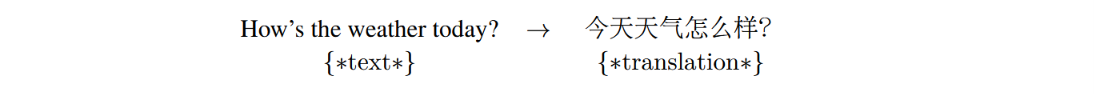
\includegraphics[width=0.8\textwidth]{_files/_images/eng-cin.png}
    \label{fig:self-instruct}
\end{figure}
\\
Possiamo generare a fine-tuning sample usando il template che abbiamo appena creato in questo modo:
\begin{figure}[h]
    \centering
    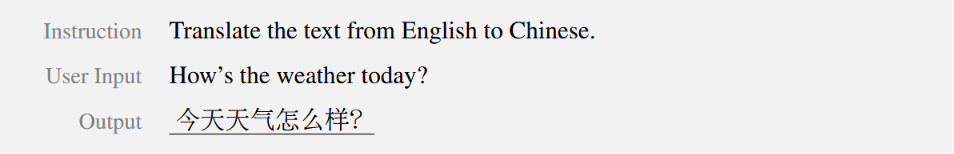
\includegraphics[width=0.8\textwidth]{_files/_images/cin_cen.png}
    \label{fig:self-instruct}
\end{figure}


Che corrisponde a:
\begin{itemize}
    \item $x$ = Translate the text from English to Chinese. How's the weather today?
    \item $y$ = "frase giapponese"
\end{itemize}
E questa coppia andrà nel dataset di fine-tuning.



\begin{observation}{Difficoltà nella creazione dei prompt template}

La principale difficoltà nella costruzione di un dataset per il
Supervised Fine-Tuning (SFT) non consiste nel riempire i template
con gli esempi disponibili, ma nel \textbf{progettare prompt template
chiari, coerenti e capaci di rappresentare correttamente il task}.

In particolare, emergono due problematiche principali:

\begin{itemize}
    \item \textbf{Uno stesso task può essere descritto attraverso
    template differenti.}

    Ad esempio, il task di traduzione dall'inglese al cinese può
    essere espresso mediante istruzioni diverse.

    Annotatori differenti possono produrre istruzioni con livelli
    di qualità e complessità differenti. Alcune potrebbero risultare
    troppo lunghe, ambigue o inutilmente complesse.

    \item \textbf{Alcuni task sono difficili da identificare
    e descrivere correttamente.}

    In determinati casi, non è immediato comprendere quale
    operazione debba eseguire il modello oppure come trasformarla
    in un'istruzione chiara e precisa.
\end{itemize}

\textbf{Possibile soluzione:}

Una strategia consiste nel partire da \textbf{task e benchmark NLP
già esistenti}, che forniscono descrizioni dei compiti ed esempi
annotati.

Gli annotatori possono quindi utilizzare queste informazioni
per formulare istruzioni appropriate per gli LLM.

Tuttavia, questo approccio richiede comunque:

\begin{itemize}
    \item Linee guida per gli annotatori;
    \item Un formato condiviso per i prompt template;
    \item Strumenti per gestire il processo di annotazione
    e crowdsourcing;
    \item Procedure di controllo della qualità.
\end{itemize}

\textbf{Conclusione:}

Una volta definiti correttamente i prompt template, è possibile
generare automaticamente numerosi esempi di fine-tuning,
sostituendo i campi dei template con gli input e gli output
dei dataset annotati.

Pertanto, \textbf{la difficoltà principale risiede nella
progettazione dei template}, mentre la generazione degli esempi
SFT diventa un processo relativamente semplice e automatizzabile.

\end{observation}


\paragraph{Dati naturalmente disponibili sul Web.}
Un'altra possibilità nella generazione manuale consiste nell'utilizzare
dati già presenti su Internet.

Per esempio, le coppie domanda--risposta raccolte
da siti di Question Answering possono essere impiegate
per l'open-domain QA.

Il vantaggio è che la varietà delle domande reali
supera quella che un piccolo gruppo di annotatori
potrebbe immaginare autonomamente.
Queste risorse possono quindi offrire quantità
e qualità dei dati adeguate.

\paragraph{Crowdsourcing di richieste reali.}
Un ulteriore approccio consiste nel consentire
agli utenti di inserire liberamente delle domande.
Le risposte possono essere:

\begin{itemize}
    \item scritte direttamente da annotatori umani;

    \item generate da un LLM e poi annotate,
    corrette o revisionate manualmente.
\end{itemize}

In questo modo si raccolgono richieste vicine
all'utilizzo reale e si includono problemi
non coperti dai task NLP tradizionali.

\paragraph{Diversità dei dati.}
La diversità è un requisito trasversale alla costruzione
dei dataset. Il testo riporta che una maggiore varietà
di prompt e task può migliorare la robustezza
e la capacità di generalizzazione degli LLM.

\subsubsection{Automatically Generated Data}
La generazione manuale dipende dall'esperienza
e dalla creatività degli annotatori.
Può risultare costosa, poco efficiente,
limitata nella copertura e soggetta ai loro bias.

Un approccio alternativo consiste nel generare automaticamente i dati di Fine-Tuning. Ad esempio, è possibile \textbf{raccogliere un insieme di domande} attraverso il crowdsourcing e \textbf{utilizzare un LLM opportunamente ottimizzato (well-tuned LLM) per generare le relative risposte}.

Le coppie domanda-risposta (question-answer pairs) così ottenute vengono successivamente utilizzate come campioni di Fine-Tuning, seguendo la procedura standard.

Questo metodo, pur essendo molto semplice, è stato ampiamente utilizzato per generare dataset di Fine-Tuning su larga scala per gli LLM.

Questa procedura è simile alla
\textbf{data augmentation}: un modello produce
predizioni per molti input, consentendo di costruire
un dataset più ampio.


Ripetendo questo processo per input differenti ci permette di creare un numero sufficiente di esempi per il fine-tuning.


Il metodo è particolarmente utile per adattare
un nuovo modello mediante un LLM già ben ottimizzato.
Resta però il limite di dipendere da input
scritti o raccolti manualmente, che potrebbero essere inappropiati per generalizzare un LLM.


In molte applicazioni degli LLM, una delle principali difficoltà deriva dalla grande varietà di domande e richieste degli utenti, molte delle quali non sono contemplate nei task e nei dataset NLP già esistenti, quindi alcune volte, i task sono complessi, che non esistono domande già pre-impostate.
In questi casi, diventa quindi necessario generare non soltanto le risposte (predictions), ma anche gli input stessi, ovvero le domande e le richieste da fornire al modello.



Qui consideriamo \textbf{self-instruct} come un esempio per illustrare come generare LLM fine-tuning samples in modo automatico.
\begin{definition}{Self-instruct}
\textbf{Self-Instruct} è una procedura che consente di generare
automaticamente esempi di Fine-Tuning, utilizzando un LLM
per produrre sia gli input sia i relativi
output (risposte).

In questo modo, è possibile costruire un \textbf{dataset sintetico}
di coppie input-output, da utilizzare successivamente
per il Supervised Fine-Tuning (SFT).
\end{definition}

Il procedimento descritto nel libro comprende
i seguenti passaggi.

\begin{enumerate}
    \item \textbf{Inizializzazione del task pool.}

    Si costruisce un insieme iniziale di task
    scritti manualmente. Ogni task contiene
    un'istruzione e un esempio input--output.
    Quindi ogni task rappresenta un sample, di quello che sarà poi il dataset finale di fine-tuning.


    \textbf{Si parte quindi da un insieme iniziale di istruzioni scritte da esseri umani (seed instructions)}


    \item \textbf{Campionamento delle istruzioni.}

    A ogni iterazione si seleziona un piccolo numero
    di istruzioni dal pool. Per favorire la diversità,
    si possono combinare istruzioni umane
    e istruzioni generate dal modello (perchè generate dal modello? lo vedrai nel prossimo punto).

    \item \textbf{Generazione di una nuova istruzione.}

    Le istruzioni selezionate vengono usate come esempi dimostrativi. Cosi l'LLM
    può fare In-Context Learning da questi esempi dimostrativi e produrre una nuova istruzione.
    Il modello riceve la richiesta di produrre
    una nuova istruzione.

    Un template (in italiano), for prompting an LLM, è il seguente:
    \begin{quote}
    Sono fornite alcune istruzioni per eseguire task diversi.
    Genera una nuova istruzione sulla base di questi esempi.

    Task 1: \texttt{\{istruzione1\}}

    Task 2: \texttt{\{istruzione2\}}

    Task 3: \texttt{\{istruzione3\}}

    Task 4: \texttt{\{istruzione4\}}

    Nuovo task:
    \end{quote}

    Verra quindi generata la nuova istruzione.

    \item \textbf{Generazione dell'esempio.}

    Data la nuova istruzione, il modello deve completare il sample da mettere nel dataset manca quindi la parte di input dell'utente, e l'output. Si genera cosi l'input dell'utente
    e l'output corrispondente facendo un prompt all'LLM.

    Un template è:
    \begin{quote}
    Sono forniti alcuni samples, ciascuno composto
    da un'istruzione, un input e un output.
    Genera un nuovo esempio sulla base di quelli forniti.

    Sample 1: \texttt{\{istruzione1\}}

    Input: \texttt{\{input1\}}

    Output: \texttt{\{output1\}}

    Sample 2: \texttt{\{istruzione2\}}

    Input: \texttt{\{input2\}}

    Output: \texttt{\{output2\}}

    Nuovo esempio: \texttt{\{nuova-istruzione\}}
    \end{quote}
    L'LLM completerà il sample, da mettere eventualmente nel dataset di fine-tuning, generando input e output.
    \begin{observation}{}
            I sample dati all'LLM, sono relativi alle istruzioni che abbiamo samplato.
    \end{observation}

    \item \textbf{Filtraggio e aggiornamento.}

    Regole euristiche controllano il nuovo esempio.
    Si possono scartare campioni non validi,
    di qualità insufficiente o troppo simili
    a quelli già presenti.

    \textbf{Gli esempi accettati e le relative istruzioni
    vengono aggiunti al pool}.
\end{enumerate}

Il processo viene ripetuto fino a ottenere
una quantità sufficiente di dati.

\begin{figure}[h]
    \centering
    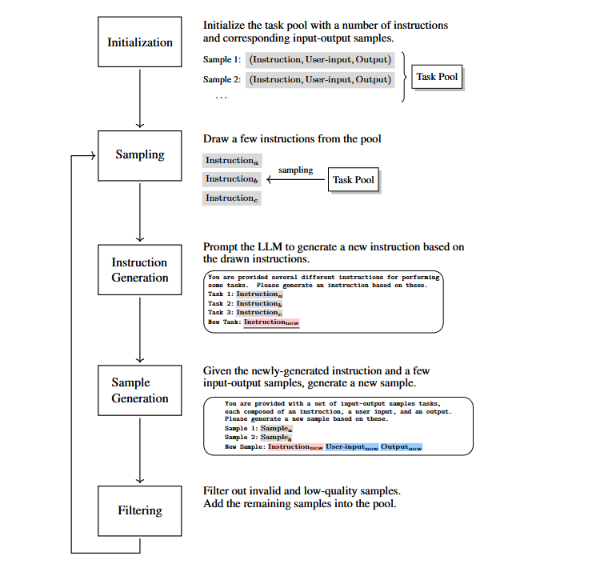
\includegraphics[width=0.5\textwidth]{_files/_images/algoritm.png}
    \caption{Procedura self-instruct. Un task pool iniziale
    contiene istruzioni ed esempi scritti manualmente.
    Alcune istruzioni vengono campionate e utilizzate
    per generarne di nuove; il modello produce quindi
    i relativi input e output. Il filtraggio elimina
    gli esempi inadeguati e quelli accettati rientrano
    nel pool. La figura evidenzia il carattere iterativo
    della costruzione del dataset.}
    \label{fig:self-instruct}
\end{figure}


\newpage


\paragraph{Impieghi dei dati sintetici.}
I dati sintetici sono ampiamente utilizzati
perché costruire manualmente grandi dataset
può superare le risorse di molti gruppi di ricerca.

Il testo menziona:

\begin{itemize}
    \item dataset di Fine-tuning che includono dati sintetici,
    come nei lavori di Ouyang et al.\ (2022),
    Taori et al.\ (2023) e Chiang et al.\ (2023);

    \item algoritmi evolutivi per aumentare
    la diversità delle istruzioni,
    come in Xu et al.\ (2024);

    \item l'impiego di dati sintetici come segnali
    di supervisione in procedure di Fine-tuning
    più articolate, come in Chen et al.\ (2024b);

    \item l'impiego di dati sintetici anche
    durante il Pre-training, come nei lavori
    di Gunasekar et al.\ (2023)
    e Allal et al.\ (2024).
\end{itemize}

\paragraph{Bootstrapping da un insieme iniziale ridotto.}
In un dominio specifico si può raccogliere
un piccolo insieme di domande e risposte
scritte da esperti.

Quando quantità e varietà non sono sufficienti,
self-instruct permette di generare ulteriori esempi
a partire da questo insieme iniziale,
ampliando il dataset.


\newpage
\subsubsection{Fine-tuning con meno dati}

La diffusione dell'Instruction Fine-tuning ha aumentato
la domanda di dataset grandi e di qualità elevata.
Il libro riporta l'esempio di \textbf{FLAN},
che raccoglie circa \textbf{15 milioni di esempi}
provenienti da \textbf{1\,836 task}.

L'addestramento su dataset di queste dimensioni
è costoso. Inoltre, una grande quantità
di dati sintetici non esclude la presenza
di errori e bias.

Il testo distingue due direzioni complementari:

\begin{itemize}
    \item rendere più efficiente l'aggiornamento del modello,
    per esempio modificando soltanto una parte
    dei parametri;

    \item ridurre i dati elaborati, selezionando
    gli esempi più pertinenti e utili.
\end{itemize}

\paragraph{Selezione di esempi ad alto valore.}
Zhou et al.\ (2023a) costruiscono un dataset
di appena \textbf{1\,000 esempi}, con prompt
curati e campioni provenienti da diversi task NLP.

Secondo i risultati riportati dal libro,
un \textbf{LLaMA 65B} adattato con questo dataset
può risultare competitivo con modelli sottoposti
a un Fine-tuning molto più esteso,
e in alcuni confronti superarli.

Chen et al.\ (2024a) utilizzano invece un sistema
basato su \textbf{GPT-3.5} per valutare la qualità
degli esempi disponibili e selezionare quelli migliori,
ottenendo risultati migliori con meno campioni.

Altre strategie comprendono:

\begin{itemize}
    \item selezione o filtraggio mediante euristiche,
    come nei lavori di Zhao et al.\ (2024)
    e Ge et al.\ (2024);

    \item assegnazione di priorità ai dati
    che influenzano maggiormente il Fine-tuning,
    come in Xia et al.\ (2024).
\end{itemize}

Queste tecniche appartengono alle più generali
famiglie di \textbf{data selection}
e \textbf{data filtering}.

\paragraph{Interpretazione: attivare capacità già apprese.}
Il fatto che pochi esempi possano essere sufficienti
si discosta dall'idea secondo cui task complessi
richiedano necessariamente grandi quantità
di nuovi dati supervisionati.

Una possibile spiegazione è che il Pre-training
abbia già fornito al modello le capacità necessarie,
ma che le risposte conformi alle istruzioni
non siano ancora quelle maggiormente probabili
durante l'Inference.

Il Fine-tuning può allora modificare moderatamente
la distribuzione degli output, rendendo più probabili
i comportamenti desiderati.

\begin{definition}{Superficial Alignment Hypothesis}
La Superficial Alignment Hypothesis sostiene che
l'apprendimento delle conoscenze e delle capacità
fondamentali avvenga principalmente durante
il Pre-training, mentre il successivo Alignment
modifichi soprattutto il modo in cui tali capacità
vengono espresse, senza contribuire in misura
sostanziale alla base di conoscenze del modello.
\end{definition}

Si tratta di un'ipotesi interpretativa:
il testo la utilizza per spiegare perché
un adattamento efficace possa richiedere
molto meno lavoro del Pre-training.

\paragraph{Chiarimento intuitivo.}
Il modello potrebbe già possedere le conoscenze
necessarie per rispondere a una domanda.
SFT può soprattutto insegnargli che, davanti
a una richiesta, deve produrre una risposta
nel formato desiderato anziché continuare
il testo del prompt.

\paragraph{Fine-tuning sulle sole risposte.}
Il testo osserva inoltre che il Fine-tuning
non deve necessariamente essere limitato
a coppie istruzione--risposta.

Hewitt et al.\ (2024) riportano che
l'Instruction-following può emergere implicitamente
anche adattando un LLM sulle sole risposte,
senza fornire le istruzioni corrispondenti.

\begin{definition}{Sample efficiency}
Un metodo di apprendimento è sample efficient
se riesce ad apprendere efficacemente
da un numero ridotto di esempi di addestramento.
\end{definition}

In questo senso, l'Instruction Fine-tuning
può essere considerato sample efficient
rispetto al Pre-training.

Il testo collega la sample efficiency
a un uso efficace di dati scarsi
e a modalità efficienti di campionare
lo spazio dei dati.

Questo principio può essere utile anche
nel Reinforcement Learning e nell'Human Preference
Alignment, sia per campionare efficientemente
dati di preferenza mediante Reward Model,
sia per migliorare il campionamento
durante l'apprendimento della Policy.

\subsubsection{Instruction Generalization}

Nel normale apprendimento supervisionato
si desidera che un modello funzioni bene
su nuovi esempi dello stesso task.

Nell'Instruction Fine-tuning si richiede qualcosa
di ulteriore: il modello deve rispondere correttamente
sia a nuovi input sia a istruzioni relative
a task differenti.

\paragraph{Notazione.}
Il testo considera un modello
\[
\Pr(y\mid c,z),
\]
dove:

\begin{itemize}
    \item $c$ è l'istruzione;

    \item $z$ è l'input dell'utente;

    \item $y$ è l'output.
\end{itemize}

Le prestazioni vengono indicate come
\[
\operatorname{Performance}\bigl(\Pr(y\mid c,z)\bigr),
\]
oppure, in forma abbreviata, con
\[
\mathcal{P}(c,z,y).
\]

Il simbolo $\mathcal{P}$ indica quindi
una \textbf{misura di prestazione},
non una probabilità.

\paragraph{Generalizzazione all'interno di un task.}
Fissata un'istruzione $c^{*}$,
si considera un insieme $Z$ di nuovi input.

Il testo descrive informalmente la generalizzazione
mediante una soglia $\epsilon$ tale che
\[
\frac{1}{|Z|}
\sum_{z'\in Z}
\mathcal{P}(c^{*},z',y')
>
\epsilon.
\tag{4.8}
\]

Qui $z'$ è un nuovo input e $y'$ il relativo output.

L'istruzione resta fissa, mentre cambiano
gli esempi sui quali viene eseguito il task.

\paragraph{Generalizzazione fra task.}
Se cambiano anche le istruzioni,
si considera un insieme $D$
di nuove coppie istruzione--input:
\[
\frac{1}{|D|}
\sum_{(c',z')\in D}
\mathcal{P}(c',z',y')
>
\epsilon.
\tag{4.9}
\]

In questo caso la variazione riguarda
\textbf{due dimensioni}: l'istruzione e l'input.

Le formule esprimono un criterio informale
basato sulle prestazioni medie.
Il testo non assegna un valore specifico a $\epsilon$
e non presenta tali disuguaglianze
come garanzie teoriche.

\paragraph{Esempio pratico: due forme di generalizzazione.}
Se il modello ha visto esempi di classificazione spam,
classificare una nuova email riguarda
la generalizzazione all'interno dello stesso task.

Se il modello deve invece eseguire una nuova istruzione,
per esempio estrarre dati finanziari da un rapporto,
la generalizzazione coinvolge anche il tipo di task.

\paragraph{Perché il problema è complesso.}
Intuitivamente, gestire entrambe le variazioni
potrebbe richiedere molti task e numerose coppie
input--output per ciascun task.

Tuttavia, il testo sottolinea che ottenere
Instruction-following su task nuovi
può richiedere costi molto inferiori
a quelli del Pre-training.
Una certa quantità di Instruction Fine-tuning
può già produrre capacità di trasferimento,
pur senza eliminare la necessità
di ulteriori adattamenti.

\paragraph{Prima strategia: aumentare la diversità.}
Una possibilità consiste nell'utilizzare dati
che coprano molti task e più formulazioni
delle istruzioni per ciascun task.

I primi dataset hanno trasformato task NLP esistenti
in un formato unificato. Il testo richiama
raccolte con oltre \textbf{100 task}
e più di \textbf{un milione di esempi}.

Il limite è che i task accademici
non rappresentano necessariamente
le richieste reali degli utenti.

Lavori successivi si sono quindi concentrati
su problemi più pratici, includendo dimostrazioni
e risposte articolate prodotte da modelli
State of the Art per richieste reali,
come nei lavori di Wang et al.\ (2023c)
e Teknium (2023).

\paragraph{Scaling dell'Instruction Fine-tuning.}
L'ampliamento dei dataset è collegato
alla più generale idea di scalare gli LLM
lungo diverse dimensioni.

Le scaling laws hanno motivato lo sviluppo
di modelli adattati con dataset più estesi.
Tuttavia, aumentare la scala del Fine-tuning
non è necessariamente il modo più efficiente
per ottenere generalizzazione nell'Alignment.

\paragraph{Limiti della sola supervisione input--output.}
SFT apprende associazioni fra istruzioni e risposte,
ma incontra difficoltà nel rappresentare
preferenze sottili o complesse, quali:

\begin{itemize}
    \item tono;

    \item stile;

    \item qualità soggettiva della risposta.
\end{itemize}

Questi aspetti sono difficili da codificare
completamente in esempi espliciti.
Inoltre, la generalizzazione resta condizionata
dalla qualità e dalla diversità del dataset.

Il testo motiva così l'impiego di modelli
di preferenza come ulteriore fase di adattamento
dopo l'Instruction Fine-tuning.

\paragraph{Seconda prospettiva: ruolo del Pre-training.}
Alcune associazioni istruzione--risposta
potrebbero essere già state apprese
durante il Pre-training.

Poiché spesso non si conosce precisamente
il contenuto dei dati di Pre-training,
è difficile stabilire quali associazioni
debbano essere effettivamente apprese
durante il Fine-tuning.

Ne deriva la domanda sul ruolo relativo
delle due fasi nella
\textbf{out-of-distribution generalization}.

Il testo richiama risultati secondo cui
un Pre-training su dati ampi e diversificati
migliora le prestazioni fuori distribuzione.

Se il modello ha già incontrato
una grande varietà di distribuzioni,
un Fine-tuning molto esteso potrebbe
non essere indispensabile per questo obiettivo.

Questa prospettiva motiva:

\begin{itemize}
    \item adattamenti contenuti, basati su pochi esempi
    accuratamente selezionati;

    \item metodi capaci di produrre Instruction-following
    anche senza essere progettati esplicitamente
    a tale scopo.
\end{itemize}

Il libro richiama in questo contesto
Zhou et al.\ (2023a) e Kung e Peng (2023).

\paragraph{Adattamento generale e specializzazione.}
Le due strategie principali sono quindi
l'ampliamento della diversità dei dati
e l'impiego di piccoli dataset sufficienti
ad attivare capacità già presenti.

Nella pratica, istruzioni diversificate
restano spesso utili.

Il testo osserva inoltre che un modello
adattato su un dominio specifico
può continuare a comportarsi come
un esecutore generale di istruzioni.

Per esempio, un Fine-tuning su dati matematici
non implica necessariamente che il modello
produca soltanto risposte matematiche:
può ancora generare una poesia
se l'utente lo richiede.

Questo mostra che il Fine-tuning
non modifica necessariamente la natura generale
dell'Instruction-following del modello.
Ulteriori dati diversificati possono aiutare
a indirizzarlo verso i comportamenti
specificamente desiderati.

\subsubsection{Usare modelli deboli per migliorare modelli forti}

Molti metodi di Instruction Fine-tuning
presuppongono dati annotati da esseri umani
oppure generati da modelli sufficientemente forti
da fornire una supervisione accurata.

Questa ipotesi diventa problematica
quando il modello da adattare è già molto capace,
oppure quando il task è difficile
anche per gli esperti.

Il libro propone l'esempio dell'analisi
di un documento estremamente lungo:
individuare incoerenze, bias sottili
o omissioni importanti può richiedere
una revisione estesa e costosa.

Si pone allora la domanda se sia possibile
utilizzare modelli più deboli
per supervisionare modelli più forti.

\begin{definition}{Weak-to-strong generalization}
La weak-to-strong generalization riguarda
la possibilità di migliorare un modello forte
mediante segnali di supervisione prodotti
da un modello più debole, ottenendo
una generalizzazione che superi i limiti
della supervisione ricevuta.
\end{definition}

Il problema è rilevante anche nella prospettiva
di supervisionare sistemi più capaci
degli esseri umani o degli altri sistemi disponibili.
Il testo precisa che non esistono ancora
soluzioni mature e generali,
pur riportando risultati promettenti.

\paragraph{Fine-tuning su predizioni del modello debole.}
Sia $X$ una raccolta di input,
ognuno comprendente un'istruzione
e, se necessario, l'input dell'utente.

Un modello debole $\Pr^{w}$ genera,
per ciascun $x\in X$, una predizione
\[
\hat{y}
=
\operatorname*{arg\,max}_{y}
\Pr^{w}(y\mid x).
\]

Un modello forte $\Pr^{s}_{\theta}$
viene quindi adattato sulle predizioni ottenute:
\[
\tilde{\theta}
=
\operatorname*{arg\,max}_{\theta}
\sum_{x\in X}
\log \Pr^{s}_{\theta}(\hat{y}\mid x).
\tag{4.10}
\]

Qui $\theta$ rappresenta i parametri
del modello forte da aggiornare.

\paragraph{Relazione con la Knowledge Distillation.}
La procedura trasferisce informazione
dal modello debole a quello forte,
assumendo la forma di un problema
di \textbf{Knowledge Distillation}.

Il rischio è che il modello forte
si limiti a imitare il supervisore,
riproducendone gli errori
oppure adattandosi eccessivamente
alle sue predizioni.

In tal caso, potrebbe non riuscire
a risolvere problemi che il modello debole
non sa affrontare correttamente.

Il testo riporta tuttavia risultati preliminari
di Burns et al.\ (2023a):
una supervisione di livello GPT-2,
utilizzata per adattare un modello
pre-addestrato forte come GPT-4,
può migliorare la generalizzazione
su diversi task NLP.

\paragraph{Misurazione delle prestazioni.}
Per valutare il risultato vengono introdotte
tre quantità.

\begin{definition}{Weak Performance}
La Weak Performance, indicata con $P_{\mathrm{weak}}$,
è la prestazione del modello debole sul test set
e costituisce il riferimento iniziale.
\end{definition}

\begin{definition}{Weak-to-strong Performance}
La Weak-to-strong Performance, indicata con
$P_{\mathrm{weak}\rightarrow\mathrm{strong}}$,
è la prestazione sul test set del modello forte
adattato mediante la supervisione del modello debole.
\end{definition}

\begin{definition}{Strong Ceiling Performance}
La Strong Ceiling Performance, indicata con
$P_{\mathrm{ceiling}}$,
è la prestazione sul test set del modello forte
adattato con dati ground truth,
per esempio risposte annotate da esseri umani.
Viene utilizzata come riferimento superiore
del confronto sperimentale.
\end{definition}

\begin{definition}{Performance Gap Recovered}
Il Performance Gap Recovered (PGR) misura
la frazione del divario di prestazione
fra modello debole e riferimento forte
che viene recuperata mediante
weak-to-strong Fine-tuning:
\[
\mathrm{PGR}
=
\max\left\{
0,\,
\frac{
P_{\mathrm{weak}\rightarrow\mathrm{strong}}
-
P_{\mathrm{weak}}
}{
P_{\mathrm{ceiling}}
-
P_{\mathrm{weak}}
}
\right\}.
\tag{4.11}
\]
\end{definition}

In particolare:

\begin{itemize}
    \item $\mathrm{PGR}=1$ indica il recupero completo
    del divario rispetto al riferimento;

    \item $\mathrm{PGR}=0$ indica che non è stato recuperato
    alcun miglioramento positivo rispetto al modello debole.
\end{itemize}

Il testo riporta valori di PGR intorno a
$0{,}8$ su $22$ task di classificazione NLP
nel lavoro di Burns et al.\ (2023a).

\paragraph{Chiarimento matematico.}
L'interpretazione come frazione recuperata
presuppone un divario positivo:
\[
P_{\mathrm{ceiling}}>P_{\mathrm{weak}}.
\]
Se il denominatore è nullo,
la formula non è definita.

Inoltre, il massimo con zero elimina
i valori negativi, ma non impone
un limite superiore pari a uno.
Il termine \emph{ceiling} designa qui
un riferimento sperimentale,
non un massimo matematico dimostrato.

\paragraph{Esempio pratico: interpretazione del PGR.}
Supponendo
\[
P_{\mathrm{weak}}=0{,}50,
\qquad
P_{\mathrm{ceiling}}=0{,}90,
\qquad
P_{\mathrm{weak}\rightarrow\mathrm{strong}}=0{,}82,
\]
si ottiene
\[
\mathrm{PGR}
=
\frac{0{,}82-0{,}50}{0{,}90-0{,}50}
=
0{,}8.
\]
Il modello adattato ha recuperato
l'$80\%$ del divario considerato.

Nonostante questi risultati,
il testo sottolinea che ottenere
una weak-to-strong generalization consistente
rimane un problema aperto.

\paragraph{Uso di una Knowledge Distillation loss.}
I modelli piccoli possono contribuire
all'addestramento anche senza produrre
soltanto risposte discrete.

Si può introdurre una loss che confronta
le distribuzioni dei due modelli:
\[
\mathrm{Loss}_{\mathrm{kd}}
=
\operatorname{KL}
\left(
\Pr^{w}(\cdot\mid x)
\,\Vert\,
\Pr^{s}_{\theta}(\cdot\mid x)
\right).
\tag{4.12}
\]

Il simbolo $\operatorname{KL}$ indica
la Kullback--Leibler divergence.
L'ordine degli argomenti esprime
il confronto dalla distribuzione
del modello debole verso quella
del modello forte.

Il testo combina questa loss
con l'obiettivo linguistico:
\[
\tilde{\theta}
=
\operatorname*{arg\,max}_{\theta}
\left[
\sum_{(x,y)\in D}
\log \Pr^{s}_{\theta}(y\mid x)
-
\lambda\,\mathrm{Loss}_{\mathrm{kd}}
\right].
\tag{4.13}
\]

Nella formula:

\begin{itemize}
    \item $D$ contiene coppie input--output;

    \item il primo termine favorisce
    la generazione degli output corretti;

    \item il secondo penalizza la divergenza
    rispetto al modello debole;

    \item $\lambda$ controlla l'influenza
    del termine di distillazione.
\end{itemize}

La loss della formula (4.12) dipende dall'input $x$;
nella scrittura compatta della formula (4.13)
l'aggregazione di questo contributo
sui dati è lasciata implicita.

Il metodo può essere utilizzato
nel Pre-training oppure nel Fine-tuning.
Una possibile scelta consiste
nel ridurre gradualmente $\lambda$,
così che il modello forte dipenda
sempre meno dal supervisore debole
man mano che acquisisce capacità.

\paragraph{Selezione e filtraggio mediante modelli piccoli.}
Un modello piccolo può valutare
la likelihood o la cross-entropy
di una sequenza e utilizzare tali quantità
come criteri di selezione.

Il testo propone, per esempio, di:

\begin{itemize}
    \item escludere sequenze con likelihood bassa
    o cross-entropy elevata,
    meno coerenti con la distribuzione
    appresa dal modello piccolo;

    \item dare priorità a sequenze
    con likelihood elevata
    o cross-entropy bassa.
\end{itemize}

\paragraph{Chiarimento sul criterio di selezione.}
La valutazione riflette ciò che il modello piccolo
ritiene coerente con la propria distribuzione.
Non costituisce, da sola,
una verifica indipendente della correttezza
di una sequenza.

\paragraph{Ensemble di modelli deboli.}
Un modello più forte può essere costruito
combinando più modelli piccoli
o sott modelli specializzati.

Le distribuzioni o le predizioni
possono essere aggregate attraverso:

\begin{itemize}
    \item majority voting;

    \item weighted averaging;

    \item stacking.
\end{itemize}

L'obiettivo è ricavare una predizione finale
dall'informazione complessivamente fornita
dai diversi modelli.

\paragraph{Model cascading durante l'Inference.}
Un modello piccolo, rapido ma meno accurato,
può essere affiancato a un modello grande,
più accurato ma più costoso.

Nel \textbf{model cascading}:

\begin{enumerate}
    \item il modello piccolo elabora per primo l'input;

    \item si verifica se il risultato soddisfa
    criteri di accettazione prestabiliti;

    \item se il risultato è sufficiente,
    viene utilizzato direttamente;

    \item altrimenti, l'input viene passato
    al modello grande.
\end{enumerate}

Poiché molti input possono essere gestiti
dal modello piccolo, la procedura riduce
il costo computazionale e la latenza complessiva.

\begin{figure}[h]
    \centering
    \IfFileExists{placeholder_figura_4_5.pdf}{
        \includegraphics[width=0.8\textwidth]{placeholder_figura_4_5}
    }{
        \fbox{\parbox{0.8\textwidth}{
            \centering
            \vspace{1cm}
            Segnaposto della figura 4.5
            \vspace{1cm}
        }}
    }
    \caption{Cinque modalità di utilizzo dei modelli piccoli:
    (a) generazione di dati sintetici per adattare
    un modello grande;
    (b) introduzione di una Knowledge Distillation loss;
    (c) selezione dei dati di addestramento;
    (d) combinazione di più modelli piccoli in un ensemble;
    (e) cascading durante l'Inference, con ricorso
    al modello grande quando il risultato del piccolo
    non è soddisfacente.
    La figura distingue gli interventi sull'addestramento
    dalle forme di combinazione dei modelli.}
    \label{fig:small-models}
\end{figure}

\subsection{Human Preference Alignment: RLHF}

\paragraph{Obiettivo.}
Seguire un'istruzione non garantisce
che la risposta sia coerente
con valori e preferenze umane.

Il libro propone l'esempio di una richiesta
relativa all'intrusione in un sistema informatico:
un modello che esegue letteralmente
la richiesta potrebbe produrre
una risposta indesiderata.
Un comportamento più appropriato
può richiedere di scoraggiare l'attività
e illustrarne le conseguenze.

Il problema è che tali valutazioni
dipendono dal contesto e da sfumature
difficili da esprimere completamente
mediante esempi supervisionati.
Talvolta le persone stesse non riescono
a formalizzare con precisione
le proprie preferenze.

\begin{definition}{Reinforcement Learning from Human Feedback}
Il Reinforcement Learning from Human Feedback
(RLHF) è un approccio nel quale le preferenze
umane sugli output vengono utilizzate
per addestrare un Reward Model,
che fornisce successivamente il segnale
di valutazione per ottimizzare l'LLM
mediante Reinforcement Learning.
\end{definition}

La procedura generale è:

\begin{enumerate}
    \item generare più risposte per una stessa richiesta;

    \item raccogliere preferenze umane sulle risposte;

    \item addestrare un Reward Model
    a prevedere tali preferenze;

    \item utilizzare i punteggi del Reward Model
    per aggiornare il modello linguistico.
\end{enumerate}

La differenza centrale rispetto a SFT
è che il modello viene guidato
da una valutazione delle risposte generate,
anziché soltanto dall'imitazione
di una risposta annotata.

\begin{figure}[h]
    \centering
    \IfFileExists{placeholder_figura_4_6.pdf}{
        \includegraphics[width=0.8\textwidth]{placeholder_figura_4_6}
    }{
        \fbox{\parbox{0.8\textwidth}{
            \centering
            \vspace{1cm}
            Segnaposto della figura 4.6
            \vspace{1cm}
        }}
    }
    \caption{Confronto fra SFT e RLHF.
    In SFT si massimizza la probabilità
    di una risposta annotata, confrontando
    le distribuzioni predette con i token attesi.
    In RLHF si generano risposte candidate,
    si raccolgono confronti umani e si addestra
    un Reward Model che guida il successivo
    Fine-tuning mediante Reinforcement Learning.}
    \label{fig:sft-vs-rlhf}
\end{figure}

\subsubsection{Fondamenti di Reinforcement Learning: punti principali}

Il Reinforcement Learning descrive
l'interazione fra un \textbf{Agent}
e un \textbf{Environment}.

A ogni passo, l'Agent osserva uno stato,
sceglie un'azione secondo una Policy
e riceve un reward e un nuovo stato.
L'obiettivo è apprendere una Policy
che massimizzi il reward cumulativo atteso.

Nel caso della generazione linguistica:

\begin{itemize}
    \item l'\textbf{Agent} è l'LLM;

    \item l'\textbf{Environment} è il contesto
    nel quale il modello genera output
    e riceve feedback;

    \item lo \textbf{State} $s_t$ è il contesto
    disponibile al passo $t$,
    cioè l'input $x$ e i token già generati $y_{<t}$;

    \item l'\textbf{Action} $a_t$ è il token $y_t$
    scelto al passo corrente;

    \item il \textbf{Reward} $r_t$ valuta
    l'azione o la risposta prodotta;

    \item la \textbf{Policy} $\pi$ è la distribuzione
    di probabilità sui token successivi.
\end{itemize}

La corrispondenza fondamentale è
\[
\pi(a\mid s)
=
\Pr(y_t\mid x,y_{<t}).
\tag{4.14}
\]

Una \textbf{trajectory} $\tau$ è una sequenza
di stati e azioni.
Il return è il reward cumulativo lungo tale sequenza.

Il testo introduce due funzioni:

\begin{itemize}
    \item $V(s)$, che valuta il return atteso
    partendo dallo stato $s$
    e seguendo la Policy;

    \item $Q(s,a)$, che valuta il return atteso
    partendo da $s$, scegliendo inizialmente $a$
    e seguendo poi la Policy.
\end{itemize}

Un discount factor $\gamma\in[0,1]$
regola il peso attribuito ai reward futuri.

\paragraph{Reward sparsi.}
Nel contesto considerato,
il reward viene tipicamente assegnato
alla risposta completa:
\[
r_t=0 \quad \text{per }t<T,
\]
mentre il reward effettivo compare
al termine della generazione.

Il feedback è quindi \textbf{sparse},
anziché disponibile a ogni passo.

\paragraph{Policy gradient e baseline.}
I metodi di Policy Gradient aggiornano la Policy
in una direzione che aumenta
il return atteso.
Non richiedono che la funzione di reward
sia differenziabile.

Una difficoltà è l'elevata varianza
delle stime del gradiente.
Per renderle più stabili
si può sottrarre una \textbf{baseline},
che costituisce un riferimento
per valutare il risultato ottenuto.

Il beneficio riguarda la varianza
della stima del gradiente:
sottrarre una costante ai reward
non riduce, di per sé,
la loro varianza.

\paragraph{Advantage e Actor-Critic.}

\begin{definition}{Advantage}
L'Advantage misura quanto un'azione sia vantaggiosa
rispetto al valore atteso dello stato
dal quale viene eseguita:
\[
A(s_t,a_t)
=
Q(s_t,a_t)-V(s_t).
\tag{4.29}
\]
\end{definition}

Nell'\textbf{Advantage Actor-Critic (A2C)}:

\begin{itemize}
    \item l'\textbf{Actor} apprende la Policy;

    \item il \textbf{Critic} apprende la Value Function
    e contribuisce alla stima dell'Advantage.
\end{itemize}

Il testo utilizza il
\textbf{Temporal Difference error (TD error)}
per stimare l'Advantage:
\[
A(s_t,a_t)
\approx
r_t+\gamma V(s_{t+1})-V(s_t).
\]

Questa espressione viene scritta nel libro
come uguaglianza nella formula (4.31);
qui il simbolo di approssimazione
ne rende esplicito il ruolo di stima.

\paragraph{Esempio pratico: significato dell'Advantage.}
Se una scelta produce un risultato migliore
di quello atteso dal Critic,
l'Advantage è positivo e l'aggiornamento
favorisce quella scelta.

Se il risultato è peggiore del previsto,
l'Advantage è negativo e la scelta
viene sfavorita.

\begin{figure}[h]
    \centering
    \IfFileExists{placeholder_figura_4_7.pdf}{
        \includegraphics[width=0.8\textwidth]{placeholder_figura_4_7}
    }{
        \fbox{\parbox{0.8\textwidth}{
            \centering
            \vspace{1cm}
            Segnaposto della figura 4.7
            \vspace{1cm}
        }}
    }
    \caption{Interpretazione di un LLM come Policy.
    Il contesto formato dall'input e dai token precedenti
    costituisce lo stato; il token successivo
    costituisce l'azione.
    Reward e Value Function forniscono il feedback
    necessario a guidare l'apprendimento della Policy.
    La figura collega la generazione autoregressiva
    al linguaggio del Reinforcement Learning.}
    \label{fig:llm-policy}
\end{figure}

\subsubsection{Addestramento del Reward Model: punti principali}

Il Reward Model associa un punteggio scalare
a una coppia input--output:
\[
r=\operatorname{Reward}(x,y).
\tag{4.33}
\]

Il punteggio esprime quanto la risposta $y$
sia coerente con il comportamento desiderato
per l'input $x$.

\paragraph{Architettura.}
Una soluzione descritta dal testo consiste
nell'utilizzare un Transformer decoder
pre-addestrato:

\begin{enumerate}
    \item si concatena $[x,y]$;

    \item si estrae dall'ultimo layer
    la rappresentazione dell'ultima posizione,
    $\mathbf{h}_{\mathrm{last}}$;

    \item una trasformazione lineare produce
    il reward:
    \[
    r(x,y)
    =
    \mathbf{h}_{\mathrm{last}}\mathbf{W}_{r}.
    \tag{4.34}
    \]
\end{enumerate}

La rappresentazione ha dimensione $d$
e $\mathbf{W}_{r}$ ha dimensione $d\times 1$.

Nel caso di reward sparsi,
la valutazione significativa viene assegnata
alla fine della risposta completa.

\begin{figure}[h]
    \centering
    \IfFileExists{placeholder_figura_4_8.pdf}{
        \includegraphics[width=0.8\textwidth]{placeholder_figura_4_8}
    }{
        \fbox{\parbox{0.8\textwidth}{
            \centering
            \vspace{1cm}
            Segnaposto della figura 4.8
            \vspace{1cm}
        }}
    }
    \caption{Architettura del Reward Model
    basato su Transformer decoder.
    L'input e la risposta vengono concatenati;
    la rappresentazione dell'ultima posizione,
    corrispondente al token finale,
    viene trasformata linearmente
    in un reward scalare.
    La figura mostra come adattare
    un modello linguistico a una funzione di scoring.}
    \label{fig:reward-model}
\end{figure}

\paragraph{Raccolta delle preferenze.}
Per ogni input si generano più risposte candidate.
Il feedback umano può assumere la forma di:

\begin{itemize}
    \item \textbf{Pairwise Comparison}:
    scelta della risposta migliore fra due;

    \item \textbf{Rating}:
    assegnazione di un punteggio
    continuo, discreto o binario;

    \item \textbf{Listwise Ranking}:
    ordinamento di un insieme di risposte.
\end{itemize}

Il testo si concentra sui confronti a coppie.
La notazione
\[
y_a\succ y_b
\]
indica che $y_a$ è preferita a $y_b$.

\paragraph{Modello di Bradley--Terry.}
La probabilità di preferire $y_a$
viene modellata come
\[
\begin{aligned}
\Pr(y_a\succ y_b\mid x)
&=
\frac{e^{r(x,y_a)}}
{e^{r(x,y_a)}+e^{r(x,y_b)}}\\
&=
\operatorname{Sigmoid}
\bigl(r(x,y_a)-r(x,y_b)\bigr).
\end{aligned}
\tag{4.35}
\]

Conta quindi la differenza fra i punteggi:
una differenza maggiore a favore di $y_a$
produce una probabilità di preferenza più alta.

Il Reward Model viene addestrato
minimizzando la negative log-likelihood
delle preferenze annotate:
\[
L_r(\phi)
=
-
\mathbb{E}_{(x,y_a,y_b)\sim D_r}
\left[
\log \Pr_{\phi}(y_a\succ y_b\mid x)
\right].
\tag{4.36}
\]

Qui $D_r$ è il dataset di preferenze
e $\phi$ comprende i parametri
del Transformer e della trasformazione lineare.

Dopo l'addestramento, il modello assegna
punteggi alle singole coppie $(x,y)$:
non è necessario presentargli sempre
due risposte contemporaneamente.

\subsubsection{Addestramento dell'LLM: punti principali}

Il Reward Model addestrato viene utilizzato
per ottimizzare la Policy.

In questa fase è sufficiente disporre
di un dataset di input:
le risposte vengono generate dal modello
e valutate tramite il Reward Model.

La procedura Actor-Critic utilizza
i reward e le stime del Critic
per favorire le scelte con Advantage positivo
e sfavorire quelle con Advantage negativo.

\paragraph{Importance sampling.}
Il testo introduce un confronto
fra la Policy corrente $\pi_{\theta}$
e una Policy di riferimento
$\pi_{\theta_{\mathrm{ref}}}$,
attraverso il rapporto
\[
\frac{\pi_{\theta}(a_t\mid s_t)}
{\pi_{\theta_{\mathrm{ref}}}(a_t\mid s_t)}.
\]

Questo rapporto permette di pesare le azioni
in base a quanto siano probabili
nella Policy corrente rispetto a quella
utilizzata come riferimento.

Se il rapporto è maggiore di uno,
l'azione è diventata più probabile;
se è minore di uno,
è diventata meno probabile.

\paragraph{PPO e stabilità degli aggiornamenti.}
La \textbf{Proximal Policy Optimization (PPO)}
mira a migliorare la Policy
evitando aggiornamenti eccessivi.

Ad alto livello, il procedimento combina:

\begin{itemize}
    \item il rapporto fra Policy corrente
    e Policy di riferimento;

    \item l'Advantage delle azioni;

    \item un meccanismo di \textbf{clipping}
    per contenere gli effetti
    di variazioni troppo ampie;

    \item una penalizzazione dello scostamento
    dalla Policy di riferimento.
\end{itemize}

La logica delle \textbf{trust region}
è mantenere gli aggiornamenti
in una zona nella quale l'ottimizzazione
resti sufficientemente stabile.

\paragraph{I quattro modelli coinvolti.}
La configurazione descritta richiede
quattro componenti basati sul Transformer decoder:

\begin{enumerate}
    \item \textbf{Reward Model} $r_{\phi}$:
    apprende dalle preferenze umane
    e valuta le coppie input--output.

    \item \textbf{Value Model} $V_{\omega}$:
    stima il return atteso a partire
    dallo stato corrente.

    \item \textbf{Reference Model}
    $\pi_{\theta_{\mathrm{ref}}}$:
    fornisce la Policy di riferimento
    per il campionamento e per il calcolo
    dell'obiettivo di addestramento.
    Nella procedura descritta viene mantenuto fisso.

    \item \textbf{Target Model o Policy}
    $\pi_{\theta}$:
    è l'LLM che viene effettivamente
    ottimizzato mediante RLHF.
\end{enumerate}

\paragraph{Ordine delle operazioni.}
La sequenza operativa presentata dal libro è:

\begin{enumerate}
    \item inizializzare i modelli:
    Reward Model e Value Model possono derivare
    da un LLM pre-addestrato;
    Reference Model e Policy possono derivare
    da un modello già adattato mediante SFT;

    \item raccogliere dati di preferenza umana
    e addestrare il Reward Model;

    \item utilizzare il Reward Model addestrato
    per ottimizzare congiuntamente
    Value Model e Policy;

    \item aggiornare il Value Model
    minimizzando una Mean Squared Error
    fra il target di valore
    e il valore predetto;

    \item aggiornare la Policy
    mediante l'obiettivo PPO.
\end{enumerate}

Reward Model e Value Model svolgono ruoli distinti:
il primo attribuisce una valutazione alla risposta;
il secondo stima il return atteso
da uno stato della generazione.

\begin{figure}[h]
    \centering
    \IfFileExists{placeholder_figura_4_9.pdf}{
        \includegraphics[width=0.8\textwidth]{placeholder_figura_4_9}
    }{
        \fbox{\parbox{0.8\textwidth}{
            \centering
            \vspace{1cm}
            Segnaposto della figura 4.9
            \vspace{1cm}
        }}
    }
    \caption{Schema complessivo di RLHF.
    Nella prima fase, i dati di preferenza umana
    addestrano il Reward Model mediante
    un obiettivo basato sul modello di Bradley--Terry.
    Nella seconda fase, un dataset di soli input
    alimenta la generazione delle risposte.
    Il Reference Model resta fisso;
    Reward Model e Value Function contribuiscono
    alla valutazione delle azioni.
    La Policy viene aggiornata mediante PPO
    e il Value Model mediante Mean Squared Error.
    La figura chiarisce le dipendenze
    fra le quattro componenti.}
    \label{fig:rlhf-completo}
\end{figure}